%------------------------------------------------------------------------
% Chapter:  Experimental data conversion 
%------------------------------------------------------------------------

\chapter{Experimental data treatment \label{data}}

This chapter illustrates the capabilities of \Discus to treat experimental
data for further analysis.

\section{Powder PDF \label{data-pdf}}

The atomic pair distribution function (PDF) can be obtained from
powder diffraction data and is a valuable tools for the study of the
{\it local} atomic arrangements in a material. This section 
describes how \Discus can be used to transform an experimental powder
diffraction pattern to a powder PDF.

The commonly used powder PDF is obtained from the reduced normalized 
intensity via a sine Fourier transform.

\begin{equation}
  G_{obs}(r) = \frac{2}{\pi} \int_{Q_{min}}^{Q_{max}}  F(Q) sin(Qr) dr
  \label{eq_f2gr}
\end{equation}

where F(Q) is obtained from the normalized intensity as:
 
\begin{equation}
  F(Q)       = Q [ S(Q) - 1 ] 
\end{equation}

The normalized intensity in turn is generated from the experimental
powder diffraction pattern through the application of several corrections. 
These corrections treat aspects like treat inelastic scattering etc.

For quite some time now, empirical corrections are used that turn out to
perform a good job, see \cite{bifa2013} for more detaiuled discussion. 
The algorithm in \Discus essentially performs along the lines described 
in \cite{bifa2013}.

\subsection{Treatment of powder data in \Discus \label{data-pdf-treat}}

The experimental powder pattern is transformed within \Discus by performing
the following steps:

First the input data are transformed onto an equidistant grid in Q-space.
The same is done for background data, if the user provided a background 
measurement. The initial steps along Q for the powder pattern and the 
background pattern do not have to be identical. The only two requirements 
are that
Q$_{min}$ of the powder data is equal or lower than the corresponding 
limit for the powder data. And secondly that the background Q$_{max}$
is higher that the limit for the data.

If background data are provided, these are subtracted from the powder
intensities. An optional scale factor allows to take different counting 
times into account.

\begin{equation}
  I_p (Q) = I_{obs} * scale \cdot Background
\end{equation}

Next \Discus calculates the average form factors squared 
$\langle f \rangle^2$, using 
the composition provided by the user or alternatively the composition of the
current structure. This step is essential, as it is the only multiplicative
correction that is applied. The user should ensure that the composition is
correct or at least close to the actual composition.

\begin{equation}
  I_i (Q) = \frac {I_{p}} {\langle f \rangle^2}  
\end{equation}

The result is point wise multiplied by Q to obtain an intermediate step 
towards F(Q). 

\begin{equation}
  F_i (Q) = Q \cdot  I_{i}(Q) 
\end{equation}

The next step is the empirical transformation into the actual F(Q). A 
polynomial function is fitted through these intermediate
data. The order of the polynomial can be adapted by the user. The 
difference between the intermediate data and the polynomial is taken as
F(Q). As the order of the polynomial should be kep moderately low, the 
polynomial itself is a slowly varying function in reciprocal space. Its 
highest frequency is much lower than that of the actual diffraction signal by 
the sample.

\begin{equation}
  F(Q) = F_i (Q) - \sum_i p_i  \cdot Q^i
\end{equation}

At this point the Q-scale can be adapted, which is likely necessary for 
electron diffraction data only. As the effective camera length might vary
slightly, \Discus allowes to determine the peak position of a significant 
maximmum in F(Q) and to scale the Q-axis with a multiplicative operation 
to set the peak position to a user provided expected value. Be aware that
this scaleing operation effectively prohibits any interpretation of 
absolute interatomic distances. Relative lengths of different pair distances
also affected by this scale.

The empirical transformation of the powder intensity onto F(Q) does not
include a transformation onto an absolute scale. Instead \Discus applies a
multiplicative operation to F(Q) to put this onto an empirically determined 
approximate absolute scale. This the integral over a peak in G(r) does not
allow you to determine an absolute coordination number. As the powder 
diffraction menu in \Discus includes a multiplicative scale factor you can
still fit the parameters of a model structure to obtain a match between 
the observed and experimental PDF.

As last step \Discus applies Eq. \ref{eq_f2gr} to obtain the observed
powder PDF. User supplied limits allow to flexibly write different 
sections of the PDF.

\subsection{Example \label{data-pdf-exa1}}

The macro in this example illustrates such a data transformation in \discus.

\begin{MacVerbatim}
 1 exp2pdf
 2 reset
 3 data xy, DATA/powder.inte
 4 back xy, DATA/background.inte, scale:1.0
 5 radiation xray
 6 comp comp:ZnO
 7 limits inst:30.0, fourier:29.5, qmin:0.90
 8 poly order:9
 9 qscale qobs:2.00, qcrystal:2.001
10 output gr:GROBS/sample.grobs, rmin:0.01, rmax:100.00, rstep:0.01
11 output iq:GROBS/sample.iqobs
12 output sq:GROBS/sample.sqobs
13 output fq:GROBS/sample.fqobs
14 run mode:inter
15 exit  ! Back to the main DISCUS menu
\end{MacVerbatim}

The \Discus command {\tt exp2pdf} steps into the data treatment menu.
As for all menus in \Discus the {\tt reset} command (line 2) allows you to ensure that all 
parameters are reset to their initial values at program start.

In lines 3 and 4 the experimental data and the background are read from the 
corresponding input files. \Discus can handle several input formats like
simples 2 or 4 column ASCII files, Spec type files or generic CSV type files.
See the on-line help in \Kuplot for the {\tt load} command for further details.

The empirical algorithm in \Discus can be applied to {\tt xray}, {\tt neutron}
or {\tt electron} diffraction data, simply choose the appropriate value on the 
{\tt radiation} command (line 5).

The composition is set in line 6 with {\tt comp} command. You can specify the 
actiul composition either with the optional parameter {\tt comp:} followed 
by a chemical statement or likewise just as a simple parameter on the 
{\tt comp} command line. The composition should be specified as a list of
atom names, optionally followed by the (relative) abundance. At names must have
a capital first letter and a lower case second letter. Spaces are irrelevant. 
Internally \Discus normalizes the sum of all element abundances to 1.
Thus the following lines would give exactly the same composition:  

\begin{MacVerbatim}
comp comp:Zno
comp comp:Zn1.0O1.0
comp comp:Zn 1.0 O 1.0
comp Zn 2 O 2.0
\end{MacVerbatim}

Alternatively you can use the current structure with in \Discus to specify the 
composition, in this case the command should be:

\begin{MacVerbatim}
comp comp:current
\end{MacVerbatim}

As data at high Q values might be affected by high noise level and detector 
artefacts, \Discus allows yo to limit the upper Q-value to an {\tt instrumental}
value on the {\tt limits} command line. Data above this Q-value will  be 
ignored and have no effect on the calculations. 

To avoid unnecessary Fourier termination ripples, the sine-Fourier transform
of Eq. \ref{eq_f2gr} should be limited at a Q$_{max}$ where F(Q$_{max}$) is zero. 
\Discus will teremine such a Q$_{max}$ value either below Q$_{max;inst}$ or
close to a user supplied value on the {\tt fourier:} parameter.

The lower limit Q$_{min}$ in the integeral, Eq. \ref{eq_f2gr} usually is less
critical. Most of the times \Discus can determine this value automatically 
as the first significant minimum in F(Q). Data below Q$_{min}$ are replaced
by a straight line to the point Q=0; F(0) = 0.

The default polynomial extends to 7the order. An indication that this order 
is too low is a peak in the experimental G(r) at very short distance below 0.5\AA{}.
If necessary try to expand the order. As a further test, run the following macro
within \Kuplot immediately after the {\tt exp2pdf} macro is finished.
 
\begin{MacVerbatim}
fit n[1]
show
exit
\end{MacVerbatim}

As the transformation creates as last \Kuplot data set F(Q). The macro will
list the parameter values and their estimated uncertainty. Ensure that the 
highest order are still significant.

The observed PDF is always written into a default file name. Most of the
times though the user will choose a suitable file name and suitable 
limits for the distance r on a {\tt output} command line, line 10. In the 
example output data will be witten into the directory {\tt GROBS}, 
file {\tt sample.grobs}. The distance values on teh optional parameters
{\tt rmin}, {\tt rmax} and {\tt rstep} are understood as \AA{}.

If the output file name starts with the string "kuplot", the output is not
written to disk but placed into KUPLOT as last dat set.

No further output is written, unless the user explicitely states the
optional parameters {\tt iq:}, {\tt sq:} and / or {\tt fq:} with an 
appropriate output file name. These optional parameter cann all be stated on the 
same {\tt output} command line or on individual lines as in the example.

Finally the operation is performed with the {\tt run} command on line 14.
As optional parameter {\tt mode} you can specify "inter" or "silent", the 
latter being the default if the {\tt mode:} parameter is omitted. With 
{\tt mode:silent} \Discus produces no further output until the menu is finished. 

In interactive mode, intermediate data are displayed. In interactive mode,
if the optional parameter {\tt fourier:} has been omitted, \Discus allows you to 
choose this value during the calculation.

Fig \ref{data-pdf-fig1} shows the experimental intensity and background that
is displayed in interactive mode. Note that the background has not yet been scaled.
%
\begin{figure}[!b]
   \centering
   \includegraphics[scale=0.4, angle=270]{iq_initial.eps}
   \vspace*{+5mm} 
   \caption{Initial intensity and background}
   \label{data-pdf-fig1}
\end{figure}
%
Fig \ref{data-pdf-fig2} shows the final F(Q). The vertical red line mark the
lower and upper limits. The upper limit Q$_{max;fourier}$ has already been 
adjusted to a position at which F(Q$_{max;fourier}$) is zero.

The vertical green line marks the peak position used for the adjustment of the
Q-scale. As \Discus will search for the highest peak with a wide window of 
0.25\AA$^{-1}$ width, choose the highest maximum in the lower Q-range. 
%
\begin{figure}[!b]
   \centering
   \includegraphics[scale=0.4, angle=270]{fq_final.eps}
   \vspace*{+5mm} 
   \caption{Final F(Q). The lower frame shows the last 4\AA$^{-1}$ to
            choose Q$_{max;fourier}$, The vertical green line shows
            the peak postion used for the optional adjustment of the Q-scale.}
   \label{data-pdf-fig2}
\end{figure}
%

Finally Fig \ref{data-pdf-fig3} shows the final G(r). 

%
\begin{figure}[!b]
   \centering
   \includegraphics[scale=0.4, angle=270]{gr_final.eps}
   \vspace*{+5mm} 
   \caption{Final G(r). Note the absence of any Fourier ripples and the
            absence of any spurious peak in the low distance range.}
   \label{data-pdf-fig3}
\end{figure}
%

%\par

%------------------------------------------------------------------------
